%% LyX 2.0.6 created this file.  For more info, see http://www.lyx.org/.
%% Do not edit unless you really know what you are doing.
\documentclass[12pt,english]{article}
\usepackage[T1]{fontenc}
\usepackage[latin9]{inputenc}
\usepackage{geometry}
\geometry{verbose,tmargin=1in,bmargin=1in,lmargin=1in,rmargin=1in}
\usepackage{amsmath}
\usepackage{graphicx}
\usepackage{setspace}
\usepackage[authoryear]{natbib}
\usepackage{subscript}
\doublespacing

\makeatletter

%%%%%%%%%%%%%%%%%%%%%%%%%%%%%% LyX specific LaTeX commands.
%% A simple dot to overcome graphicx limitations
\newcommand{\lyxdot}{.}


\@ifundefined{date}{}{\date{}}
%%%%%%%%%%%%%%%%%%%%%%%%%%%%%% User specified LaTeX commands.
\usepackage{longtable}
\usepackage{dcolumn}
\usepackage{pdflscape}
\usepackage{graphicx}
\usepackage{endnotes}

\makeatother

\usepackage{babel}
\begin{document}
\begin{doublespace}

\title{\textbf{\large{Mass Media and the Domestic Politics of Globalization}}}
\end{doublespace}


\author{Justin Murphy%
\thanks{Lecturer at University of Southampton. Email: j.murphy@soton.ac.uk.%
}}


\date{January 30, 2014}
\maketitle
\begin{abstract}
{\normalsize{Much is known about the domestic politics of globalization
but political scientists have largely ignored one critical link between
the international economy and most individuals around the world: the
mass media. Considering the likely effects of mass media on public
perceptions of responsibility, this article develops a simple model
of the effects of mass media on individuals' blame attributions and
propensities to mobilize around the distributive conflicts of economic
globalization. These effects of mass media on perception and mobilization
alter the incentives of a national policymaker's choice either to
compensate or neglect domestic groups harmed by globalization. Individual-level
implications of the theory are tested on survey data from France in
1992-1993 and state-level implications are tested on data from most
countries around the world from 1960 to 2010. The evidence shows that
mass media demobilize groups harmed by globalization, leading to weakened
welfare-state responsiveness. }}{\normalsize \par}

{\normalsize{Word count: 7,740 with tables and graphs.}}{\normalsize \par}

{\normalsize{\newpage{}}}{\normalsize \par}
\end{abstract}
Although the relationship between economic globalization and modern
welfare states has been one of the most studied issues in political
economy over the past three decades (e.g., \citealt[316]{Gourevitch:1978bn,Garrett:1995tj,Rodrik:1998te,Burgoon:2001dp,Adsera:2002vt,Oatley:2011hv}),
recent research on public opinion and political behavior in open economies
raises serious questions about the assumptions of this tradition (\citealt[155]{Hellwig:2007wt}).
A fundamental assumption in globalization-welfare research, which
dates back to Karl Polanyi's \emph{The Great Transformation,} is that
policymakers who wish to liberalize economic markets are held accountable
by those groups who would suffer the adjustment costs (\citealt{Polanyi:2001vc,Ruggie:1982wx}).
Scholars have shown that to sustain political coalitions in favor
of opening national economies, national policymakers have to compensate
protectionist domestic groups with side payments in the form of social
welfare programs (\citealt[1028-29]{Katzenstein:1985ub,Rodrik:1998te,Adsera:2002vt}).

However, one current of research in comparative political behavior
shows convincingly that as domestic economies become increasingly
integrated, citizens perceive that governments have less ``room to
maneuver'' and accordingly shift their blame away from domestic policymakers
to the unaccountable pressures of the global economy (\citealt{Alcaniz:2010gb,Hellwig:2012vk}).
Furthermore, citizens in countries highly exposed to the global economy
are less likely to punish incumbents for a poorly performing economy
(\citealt{Hellwig:2007gn}) and more likely to base their vote on
non-economic issues (\citealt{Hellwig:2008ia}). If domestic groups
do not punish politicians for economic losses made possibile by the
political decisions to maintain open national economies, then an essential
causal link in current accounts of the globalization-welfare nexus
would appear to be broken.

At the same time, beyond objective increases in economic globalization,
previous research has shown that mass media have direct effects on
perceptions relevant to how citizens are likely to understand the
politics of globalization. Specifically, mass media have direct effects
on perceptions of responsibility (\citealt{Iyengar:1987uo}; \citealt{Iyengar:1991uf}),
the politicization of economic hardship (\citealt{Mutz:1992ww}; \citealt{Mutz:1994kp}),
and civic engagement more broadly (\citealt{Putnam:1995vj}; \citealt{Norris:2000uf};
\citealt{Hooghe:2002bi}). Certainly, these effects are still debated
and, in fact, the conventional wisdom in the political economy of
media associates robust mass media systems with government responsiveness
and accountability (\citealt{JamesMSnyder:2012th,Besley:2002tg,Adsera:2003cc}).
Yet, in the specific context of the distributive domestic politics
of globalization, the preponderance of previous research strongly
converges on a set of counter-intuitive arguments: \emph{By shifting
citizen blame attributions away from governments and toward international
forces, both economic openness and mass media reduce the ability of
domestic groups to hold national policymakers accountable for the
effects of economic openness. In turn, as the global economy and mass
media penetrate states, national policymakers face less pressure to
compensate protectionist domestic groups for economic hardships linked
to the global economy. As states become increasingly penetrated by
both the global economy and mass media, the state-level outcome is
a weakened compensatory relationship between economic openness and
welfare spending.}

These expectations are tested with survey data and state-level economic
data ideally suited to assess the implications of these arguments
at both levels of analysis. A Legidoscope survey from France in 1992-1993
provides a unique opportunity to test the argument that mass media
has independent effects on individuals' perceptions, blame attributions,
and behavior around issues of economic openness. The findings show
that mass media exposure is positively associated with individuals'
perceptions of economic openness as a problem and then, controlling
for whether economic openness is perceived as a problem, the attribution
of blame to international forces. For comparability with respect to
previous research on the globalization-welfare nexus, the state-level
implications of the theory are tested on pooled cross-sectional, time-series
data from most countries in the world between 1960 and 2010. Using
measures of information-communication technology (ICT) penetration
rates as a proxy for the prevalence of mass media within states, several
analyses across multiple model specifications suggest that the spread
of ICT and the mass media they carry is associated with a weakening
of the positive relationship between economic openness and social
welfare spending. The dampening effect of mass media holds after controlling
for several rival explanations and when included in the replication
of previous, influential studies. Consistent with the survey analysis,
the state-level associations are interpreted as evidence for the argument
that policymakers are more likely to neglect domestic groups harmed
by political decisions to liberalize markets the more prevalent is
mass media within their states. Specifically, this is because mass
media tends to shift the perceptual and behavioral response of protectionist
individuals away from blaming and acting against the government on
the politics of openness.

These findings alter the prevailing wisdom in at least three ways.
First, they provide new evidence for the claim that economic openness
makes citizens less likely to blame, and less likely to punish, incumbent
governments for poor economic performance, but they also reveal that
mass media exposure is an alternative and independent causal path
to the same effect, controlling for perceptions of economic openness.
Second, this is the first systematic investigation of mass media as
a political \emph{institution} that conditions the domestic politics
of the global economy. As such, it directly responds to calls for
more truly political accounts of the domestic effects of globalization
(\citealt[341]{Kayser:2007ig}) and for a more rigorous examination
of the micro-foundations of work in this tradition (\citealt[474]{Hays:2005vo}).
Substantively, this research highlights a source of cross-national
and temporal variation often omitted in analyses of comparative and
international political economy. State-level evidence presented here
suggests the omission of mass media has led to biased conclusions
which over-estimate the egalitarian effects of democratic institutions
in the globalization-welfare nexus. Third, this research bears important
implications for democratic representation in a globalized world.
The evidence suggests that from the standpoint of democratic theory,
mass media can have subtle but perverse effects on the distributive
politics of open economies, disempowering domestic groups from holding
national policymakers accountable for the unevenly distributed costs
of globalization.

The article proceeds as follows. In the first section, previous literature
is reviewed to reveal a gap between comparative and international
political economists on the one hand and scholars of public opinion
and political behavior on the other, and to suggest how a formidable
history of mass media research speaks directly to this gap. A second
section develops specific hypotheses regarding how mass media is likely
to affect individual perceptions, blame attributions, and propensities
to mobilize around the politics of economic openness. That section
concludes by incorporating the expected effects of mass media into
a baseline model of the globalization-welfare nexus typical of the
most influential work in this area (Adser\`{a} and Boix\citeyear{Adsera:2002vt}).
A third section discusses the data and modeling strategy, the penultimate
section discusses the core findings, and a final section concludes.


\section{{\normalsize{Mass Media Between Globalization and Domestic Politics}}}

Despite the quantity of studies on the relationship between economic
openness and the public sector, the individual-level assumptions in
this line of research remain largely untested (\citealt{Hays:2005vo},
474). At the same time, findings from various subfields in political
science together suggest that public perceptions and attributions
of blame with respect to economic openness have affected citizen's
evaluations of government, the political behavior of voters, and ultimately,
policy outcomes. Finally, apart from the effect of objective levels
of economic openness, a review of mass media research suggests how
mass media can independently affect citizen perceptions and blame
attributions around the politics of economic openness, thereby altering
the expected outcomes of globalization-welfare models.

One of the most robust findings in international and comparative political
economy is the positive state-level correlation between international
trade and size of the public sector (\citealt{Cameron:1978vb,Rodrik:1998te,Garrett:1995tj,Adsera:2002vt}).
Most political scientists theorize this regularity as \textquotedbl{}embedded
liberalism,'' exemplified in the postwar proliferation of Keynesian
social pacts that promoted open national markets with state-sponsored
social protections (\citealt{Ruggie:1982wx}). Although social scientists
widely agree that the expansion of international trade is welfare-improving
in the long run, they also agree that the construction or expansion
of markets often induces political backlash from domestic groups in
the short run. This backlash requires policymakers in favor of increasing
openness to compensate such groups through side payments, typically
in the form of redistributive social spending, lest the necessary
political support for increasing openness breaks down. In the 1940s,
Karl Polanyi first advanced this perspective in his famous notion
of the ``double movement\textquotedbl{} that characterizes market
expansions and corresponding expansions of state welfare provision
(\citealt[79, 385]{Polanyi:2001vc};). Even across much disagreement
about which aspects of economic openness have the most effect on the
various components of welfare spending (\citealt{Mares:2004el,Ansell:2008wl,Burgoon:2001dp}),
in which countries the relationship holds (\citealt{Rudra:2002ui,Anonymous:2008ur}),
and even whether the focus on economic openness per se is mistaken
(\citealt{Kim:2007wu,Oatley:2011hv}), scholars are unanimous in the
expectation that the increasing openness of national markets elicits
a corresponding political backlash from those domestic groups who
would bear the adjustment costs.

Despite the leverage it provides to most models of the relationship
between globalization and welfare-state effort, there is surprisingly
little evidence for the assumption that domestic groups harmed by
economic liberalization exert sufficient political pressure on national
policymakers that policymakers provide welfare compensation to appease
them.%
\footnote{One exception is Hays, Ehrlich, and Peinhardt\citeyearpar{Hays:2005vo},
who find evidence that government spending helps sustain support for
free trade. This does not, however, answer the very different question
of whether globalization induces in the public a demand for compensation
on its basis. Another exception is \citealt{Margalit:2011hm}, who
finds that job losses due to offshoring had a stronger negative effect
on incumbent vote share than job losses not related to offshoring.
Significantly, that study also finds that spending from the Trade
Adjustment Assistance program significantly reduced the size of the
effect. Still, it remains unclear whether and how other institutions
moderate the public perceptions and electoral consequences of liberalization
and if different dimensions of liberalization have the same domestic
effects as offshoring in particular. For instance,\citet{Guisinger:2009vt}
finds that trade policy may not be sufficiently salient, even to the
most affected groups, to justify voter-driven models of trade policy.%
} Indeed, diverse perspectives in the social sciences suggest causal
pathways through which citizens harmed by the adjustment costs of
liberalization would not hold policymakers accountable for the political
decision of liberalization.

First, research mostly from advanced democratic countries finds that
as the sources of economic growth shift, citizens accordingly adjust
their expectations of government policymaking and their attributions
of blame for national problems.%
\footnote{It should also be noted that expectations of government policymaking
and blame attributions are not only driven by material or institutional
changes in the political economy but may also be endogenous to vote
choice or the partisan composition of an incumbent government (\citealt{Wlezien:1997ia}).%
} Using time-series data from France between 1985 and 2002, Hellwig
shows that as exposure to trade and capital flows increase, citizens
becomes less confident in the ability of national policymakers to
solve national problems and the public demand for economic policy
solutions decreases (\citealt{Hellwig:2007wt}). Voters also adjust
their judgement of governments in predictable ways as other components
of the institutional context change. For instance, when the Bank of
England gained political independence, British voters were less likely
to base their evaluation of the government on monetary policy and
more likely to base it on fiscal policy (\citealt{:2010fv}). Just
as evaluations of government shift with the material and institutional
sources of economic outcomes, so too does blame for national economic
problems. In their study of seventeen Latin American countries, Alcaniz
and Hellwig (\citeyear{Alcaniz:2010gb}) show that as exposure to
international trade increases, citizens are more likely to blame international
actors and less likely to blame the government for the country's economic
problems.

Secondly, perceptions and blame attributions affect political outcomes
by altering what policymakers can be credibly held accountable for.
Analyzing all 560 democratic elections between 1975 and 2002, Hellwig
and Samuels (\citeyear{Hellwig:2007gn}) show that as trade and capital
flows increase as a share of gross domestic product, domestic economic
growth rates have a smaller effect on incumbent vote share. Cross-sectional
analyses of French and British survey data from 1997 and 2001, respectively,
show similar effects of globalization on the determinants of vote
choice, decreasing the effect of voter's economic performance evaluations
and party positions on economic issues (\citealt{Hellwig:2008ia}).
Perceptual shifts in the ability of governments to affect economic
policy also affect voter turnout. Analysis from the United States
has found that individuals who suffer the economic adversity but do
not blame the government are less likely to vote than comparable individuals
who do blame the government (\citealt{Arcenaux:2003ue}). In terms
of policymaking, elite messaging in the mass media (\citealt{Hellwig:2011iu})
and interviews with party elites in Europe (\citealt[206]{Hellwig:2012vk})
confirm that politicians consciously stress globalization constraints
on their own behavior. Additionally, changes in the institutional
setting are found to have predictable moderating effects on the responsivness
of policy to public opinion. For instance, Sattler, Brandt, and Freeman
(\citeyear{:2010fv}) show that before central bank independence,
British fiscal and monetary policies were responsive to aggregate
voting intentions and government approval ratings but, after central
bank indepedence, monetary policy was no longer responsive. Interestingly,
however, Sattler, Brandt, and Freeman \citeyearpar{Sattler:2008vw}
find mutual responsiveness between public opinion and policy \emph{outputs},
despite a lack of responsiveness in policy \emph{outcomes} such as
inflation and economic growth. That this responsiveness is observed
outside real economic outcomes is accredited to the difficulty of
identifying the effects of policies in open economies.

Given that public perceptions of the institutional context have been
shown to affect political consequences of the economy, it is puzzling
that scholarship on the domestic politics of economic globalization
has largely neglected a serious inquiry into political communication
and the mass media in particular. \emph{Prima facie}, it is hard to
believe that many individuals \emph{directly} monitor levels of economic
openness independent of some political communication channel. It is
equally hard to imagine policymakers as passive victims in globalization's
encroachment on their room to maneuver, as if room-to-maneuver constraints
are an objective development which the mass media simply reports.
Rather, scholars of American politics have shown that national policymakers
actively engage in strategies of ``blame avoidance'' through the
mass media (\citealt{Weaver:1986ku,Jacobson:1983tg}), diffusing blame
horizontally toward other equals or vertically upward in the chain
of authority (\citealt{McGraw:1990kk,McGraw:1991up}).%
\footnote{\citet[20]{Hood:2002ko}suggests that by lowering the potential costs
of communicating malign policy effects to harmed groups, mass media
may increase the incentives for politicians to avoid blame. See also\citet{Hood:2009ed}.%
} Variation in blame attributions, in turn, has predictable effects
on how individuals judge both policies and policymakers (\citealt{McGraw:1995up}).
``Indexing'' theories of news coverage suggest that the mass media
are most likely to convey elite issue-framings (\citealt{Bennett:1990bp,Zaller:1996vs,Bennett:2006gc}).
Applied to the domestic politics of globalization, an indexing theory
of news coverage suggests that mass media is more likely to publicize
the perception (which policymakers have strategic incentives to espouse)
that economic openness constrains policymaker autonomy than alternative
narratives placing responsibility on governments. Other work has shown
that under certain conditions mass media can diffuse blame through
issue framing (\citealt{Iyengar:1987uo};\citealt{Iyengar:1991uf}),
depoliticize personal experience in favor of sociotropic perceptions
(\citealt{Mutz:1992ww}), and exacerbate inequalities in political
participation (\citealt{Norris:2000uf}). More generally, a formidable
and highly critical tradition of observers have advanced richly argued
but largely untested propositions converging on the expectation of
profoundly antidemocratic tendencies in the modern mass media (\citealt{Herman:1988ta,adorno2001culture,mcchesney2000rich}).
In light of these research currents, it is a surprising omission in
previous research on the domestic politics of globalization that testimony
by party elites in research interviews (\citealt[206-07]{Hellwig:2012vk})
and via the mass media (\citealt[420-21]{Hellwig:2011iu}) is more
often cited as evidence of room-to-maneuver constraints than questioned
as possible strategic communication or media bias. Especially because
evidence for opinion-policy responsiveness in open economies can be
observed apart from and despite the objective economic effects of
policy \citep{Sattler:2008vw}, a necessary next step in studying
the domestic politics of globalization is to theorize more specifically
how political communication---in particular, the mass media---directly
and indirectly affects the relationship between objective patterns
of economic openness and domestic economic outcomes.


\section{{\normalsize{Theory and Hypotheses}}}

In this section, I deduce specific hypotheses regarding how mass media
should be expected to affect individuals' perceptions of economic
openness, blame attributions for national problems, and ultimately
the decisions of national policymakers.

A dominant theory of political news coverage suggests that elite opinion
is one of the most significant determinants of how journalists report
political issues (\citealt{Bennett:1990bp,Zaller:1996vs,Bennett:2006gc}).
Because economic globalization can be blamed on both transnational
corporations and other foreign governments (horizontal diffusion)
as well as global market pressures outside the authority of states
(vertical diffusion), we should expect national policymakers to engage
in both types of blame diffusion. If politicians indeed diffuse blame
for economic globalization, a simple indexing theory of mass media
applied to the domestic politics of globalization predicts that mass
media reports are more likely to evoke room-to-manuever constraints
than policymaker responsibility in reporting issues of economic openness.
Qualitative evidence for such indexing is already ample in previous
research on the domestic politics of globalization, which finds that
party elites consistently invoke room to maneuver constraints in research
interviews (\citealt[206-07]{Hellwig:2012vk}) and via mass media
messaging (\citealt{Hellwig:2011iu})%
\footnote{In their study of \emph{The Guardian, The Times, The Daily Telegraph,
and The Independent} from September 2008 to May 2009, Hellwig and
Coffey find that most statements from the incumbent Labor Party diffused
blame for the 2008 financial crisis toward the United States, the
global financial system, and domestic bankers, although toward the
end of the period under study the Labor Party appeared more willing
to publicly take blame. Conservatives were more likely to blame the
government than Labour. See\citealt{Hellwig:2011iu}, 420-421.%
}. Most conservatively, this suggests that mass media will have an
indirect effect on how individuals attribute blame for national problems,
by exposing individuals to the argument that economic openness constrains
the ability of policymakers to meet certain demands from the public.
A stronger version of this argument is that mass media will have a
direct effect on how individuals attribute blame for national problems,
distinct from its effect of making individuals more aware of the problems
of economic openness per se.

\emph{Hypothesis 1: Individuals more exposed to mass media are more
likely to blame international forces for national problems than individuals
less exposed to mass media. This effect is expected directly (by diffusing
political responsbility in general, controlling for perceptions of
openness as a problem) and indirectly (by increasing awareness of
openness as politically problematic).}

Hypotheses 2 and 3 capture implications of previous research suggesting
that perceptions of a policymaker's room to maneuver affect how individuals
evaluate government performance. If the effect of economic perceptions
on vote choice weakens because increasing economic openness shifts
blame attributions toward the global economy and away from governments,
then blame attributions should be associated with evaluations of government
economic performance. Thus, I hypothesize that individuals who blame
international forces for national economic problems should be more
favorable toward incumbent governments than those who blame the government. 

\emph{Hypothesis 2: Individuals who blame international forces for
national problems evaluate incumbent governments more favorably than
individuals who blame the government for national problems.}

Combining insights from research on voting in open economies and research
on voter turnout suggests that the effect of economic openness on
the decision to vote should be conditional on whether blame for economic
openness is attributed to the government. If they blame the government,
then individuals who perceive economic openness to be a national problem
should be more likely to vote than those who do not perceive openness
to be a problem. If they blame international forces, then individuals
who perceive economic openness to be a national problem should be
less likely to vote than those who do not perceive economic openness
to be a national problem.

\emph{Hypothesis 3: The effect of perceptions of economic openness
on the decision to vote should be conditional on whether blame is
attributed to the government. It should have a positive effect for
those individuals who blame the government, and a negative effect
for those who do not blame the government.}

To assess how mass media enters into models of the globalization-welfare
nexus, consider the model of Adser\`{a} and Boix \citeyearpar[231-236]{Adsera:2002vt}
as a baseline. The model explicates the conditions under which national
policymakers must provide welfare compensation to protectionist interests
in order to secure political support for opening the domestic economy.
Adser\`{a} and Boix consider an economy of three groups of identical
individuals with distinct trade interests. Groups \emph{C, P}, and
\emph{O} are groups that can be thought of as classified by factor
endowment, sector, or firm. \emph{C} is a group that prefers a closed
economy, with utility decreasing in a linear fashion as the economy
opens. \emph{O} is a group that prefers an open economy, with utility
increasing in a linear fashion as the economy opens. \emph{P} is a
group the preferences of which are contingent on the state of the
international business cycle. Formally, these preferences are written
as

\begin{equation}
\ensuremath{U_{C}=(1-\gamma)C_{C}+\gamma C_{O}}
\end{equation}


\begin{equation}
\ensuremath{\ensuremath{U_{O}=(1-\gamma)O_{C}+\gamma C_{O}}}
\end{equation}


\begin{equation}
\ensuremath{EU_{P}=(1-\gamma)P_{C}+\gamma[\pi P_{g}+(1-\gamma)P_{b}]},
\end{equation}


\noindent where \emph{C\textsubscript{C}} and \emph{O\textsubscript{C}}
are the returns to \emph{C} when the economy is closed and open, respectively;
\emph{C\textsubscript{O}} and \emph{O\textsubscript{O}} are the
returns to \emph{O} when the economy is closed and open, respectively;
P\textsubscript{C} is the return to \emph{P} when the economy is
closed; \emph{P\textsubscript{g}} is the return to \emph{P} if the
economy is open and the international business cycle is in growth;
\emph{P\textsubscript{b}} is the return to \emph{P} if the economy
is open and the international business cycle is in recession; $\pi$
is the probability the international business cycle is in growth;
and, importantly, $P_{g}>P_{c}>P_{b}$. For any \emph{$P$}, an open
economy is preferable to a closed economy: $\pi P_{g}+(1-\gamma)P_{b}<P_{c}$. 

Groups\emph{ $C$,} \emph{$P$, }$O$ choose one of two parties at
a national election. A protectionist party, $\Sigma$, receives the
votes of \emph{C} and a pro-trade party, $\Omega$, receives the votes
of \emph{O}. Neither \emph{C} nor \emph{O} represent a majority of
voters, so \emph{P} is the median and swing vote. Both parties, $\Sigma$
and $\Omega$ , credibly commit to a level of openness, $\gamma$,
and a publicly-funded compensation package, $\alpha$, for $P$ in
cases of international recession. Voters then vote.

In this model, it can be shown that to open the domestic economy under
competitive elections, a pro-trade political party must offer domestic
spending to compensate $P$ for the increased risks of international
openness (\citealt[236]{Adsera:2002vt}). \emph{P} voters vote for
the pro-trade party, $\Omega$, if the expected value of an open economy
plus the compensation package $\alpha_{O}$ promised by $\Omega$
is greater than the the expected value of a closed economy plus the
compensation package offered by$\Sigma$. Because \emph{P}'s gains
from trade are always lower than the expected gains from a closed
economy \emph{ex ante},  the pro-trade party $\Omega$ always offers
a compensation package $\alpha_{O}$ to draw $P$ voters (\citealt[236]{Adsera:2002vt}).

Because this model assumes full and equal participation of voters,
as Adser\`{a} and Boix point out in a footnote, if turnout varies
across domestic groups then the expected policy outcome changes. In
particular, it easy to see that if \emph{P} is expected not to vote,
then the pro-trade party has no incentive to offer a compensation
package. Additionally, however, the perception that economic liberalization
is a process occuring independent of political parties, has an equivalent
effect. This effect could be conceptualized as an equalization of
the value for $\gamma$ proposed by each group. The parties would
be increasingly indistinguishable in the risks of international exposure
associated with each party. As this perceived difference decreases,
the possibility of either party losing votes due to their chosen level
of openness decreases because neither party could credibly commit
to do otherwise. As a result, the original pressure to provide compensation--to
keep voters from defecting to the more protectionist party--decreases.
Thus, 

\emph{Hypothesis 4: At the state level, the interaction of economic
globalization and mass media penetration will be associated with lower
levels of domestic welfare spending than predicted by economic globalization
alone.}

\begin{center}
\begin{figure}
\begin{centering}
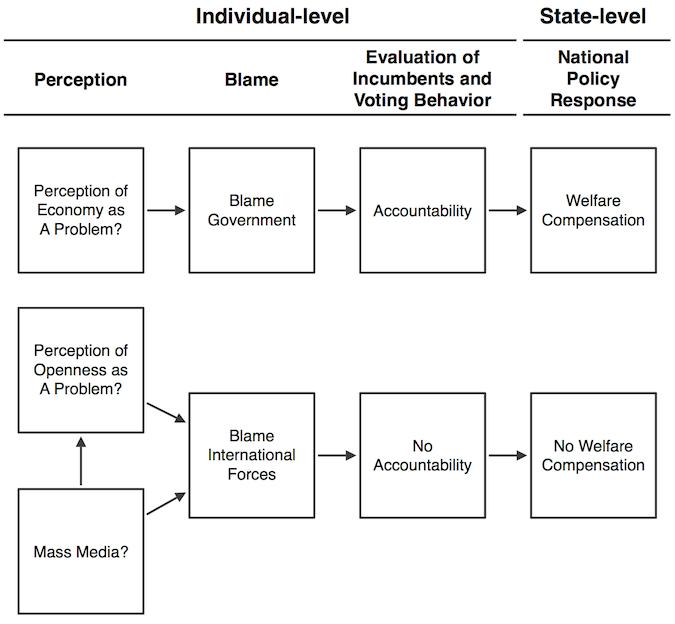
\includegraphics{Flowchart}
\par\end{centering}

\caption{Summary of the Hypothesized Effects of Perception and Mass Media in
Domestic Responses to Economic Liberalization}
\end{figure}

\par\end{center}


\section{{\normalsize{Data and Method}}}

Given the individual-level and state-level implications of the theory,
data is gathered from both levels of analysis.%
\footnote{Full summary statistics for both datasets can be found in the online
appendix.%
}The individual-level data come from a Legidoscope survey of public
opinion in France between 1992 and 1993 (\citealt{Chrique:1993us}).
Around the time of the Maastricht Treaty, especially controversial
in France, the problems of economic openness are likely to be highly
salient. Additionally, France has relatively high rates of voter turnout,
and a statist, egalitarian political culture. Thus, evidence that
mass media leads French citizens near the time of Maastricht to blame
international forces rather than their government suggests that such
a relationship is at least as likely in the many countries in which
the economy and globalization are less politicized. Similarly, if
mass media pacifies French citizens in either perceptions or political
behavior, it is likely to do so in other countries. The survey asks
respondents several questions tapping blame attribution, media exposure,
and political mobilization.%
\footnote{See the online appendix for the text of the survey questions. %
} Respondents are asked to identify their main source of information
from among the following: friends, family, opinion leaders, and mass
media. Respondents are also asked to identify the top two problems
facing France, and whether individuals, social institutions, the government,
or international forces beyond government control are to blame for
the problem.%
\footnote{Respondents were asked to identify national problems in an open-ended
fashion; their answers were then coded by the interviewer and into
the general problem types listed here. To create the binary variable
which measures whether the respondent sees some aspect of international
economic openness as a top problem, I coded respondents as 1 if they
identified one of the following issues as one of the ``second most
important problems'': ``Int\textquoteright{}l economic competition,''
``EC-92, economic integration,'' ``Foreign trade,'' ``Ratification
of Maastricht,'' and ``Maastricht Treaty.'' All other respondents
were coded as 0 for the variable $Openness\: Problem$.%
} Finally, respondents are asked about their satisfaction with President
Mitterand, how well they think the government is handling the problem
identified by the respondent as a top problem, and their intention
to turnout for the March 1993 elections.

To test the direct and indirect effects of mass media on blame (Hypothesis
1), I estimate two logistic regression models. The first estimates
the probability a respondent will blame international forces as a
function of mass media exposure and a vector of control variables
including controls for the nature of the problem. The equation is

\begin{eqnarray}
Blame_{i} & = & \alpha+\beta_{1}General\: Problem\: Type_{i}+\beta_{2}Openness\: Problem_{i}+\beta_{3}Media_{i}+ \notag \\
&  & \beta_{4}Controls_{i}+e_{i},
\end{eqnarray}

\noindent where $Blame$ is a binary variable taking a value of 1
for respondents who blame international forces and 0 for respondents
who blame the government for whichever national problem they have
identified.%
\footnote{Because of space constraints and for ease of interpretation in light
of the hypotheses under consideration, I consider here only the difference
between blaming the government and blaming international forces, omitting
respondents who placed the blame on ``society'' or ``people like
you and me.'' However, the results obtained here are robust to multinomial
specifications which include these alternative blame attributions
and alternative binary codings (included in the online appendix).%
} $General\: Problem\: Type$ is a categorical variable with four levels
indicating whether the problem deals with social, economic, political,
or foreign issues;%
\footnote{In the first wave of the survey, so many respondents identified unemployment
as the top problem facing France that a question was added to measure
what respondents identified as the ``second most important problem
facing France today.'' All the analyses here, including the variables
measuring blame attributions and evaluations of government handling,
refer to this second most important problem.%
} $Openness\: Problem$ is a binary variable I constructed to take
a value of 1 for respondents who identified a problem specifically
related to economic openness and 0 otherwise. If the mass media have
an independent effect on diffusing blame away from government policymakers
and toward international forces, then we would expect $\beta_{3}$
to be positive and significant.

Then, to assess the indirect effect of mass media on blame as its
channeled through perceptions of economic openness, I estimate a logistic
regression modeling the probability of perceiving openness as a top
problem as a function of mass media exposure and a vector of control
variables:

\begin{eqnarray}
Openness\:Problem_{i} & = & \alpha+\beta_{1}General\:Problem\:Type_{i}+\beta_{2}Media_{i}+ \notag \\
&  & \beta_{3}Controls_{i}+e_{i}.
\end{eqnarray}

where the main variables of interest are the same as in Equation 1
except that here the dependent variable is the binary variable capturing
whether openness is perceived as a top problem. If mass media affect
blame attributions indirectly by making individuals more aware of
international economic forces, which in turn would shift their blame
toward international forces, then $\beta_{2}$ should be positive
and significant.

To test Hypothesis 2 regarding the effect of blame attributions on
evaluations of the government, I estimate a linear regression modeling
how individuals evaluate the government's handling of the problem
they identified as one of the most important facing the country. I
model evaluations of government handling as a function of respondents'
blame attributions and a vector of control variables. The equation
is

\begin{eqnarray}
Gov\:Handling_{i} & = & \alpha+\beta_{1}General\:Problem\:Type_{i}+\beta_{2}Openness\:Problem_{i}+ \notag \\
&  & \beta_{3}Blame_{i} + \beta_{4}Controls_{i}+e_{i},
\end{eqnarray}

\begin{doublespace}
\noindent where $ $$GovHandling_{i}$ measures, on a scale from 1
to 4, how the \emph{i}th respondent evaluates the government's handling
of the top problem they identified. The theory predicts that for a
particular problem such as the domestic costs of economic openness,
blaming international forces rather than the government will make
individuals less likely to hold governments accountable for that problem.
If this is the case, then individuals who think a problem is caused
by forces outside of the government's purview should be less critical
of the government's handling of that problem. In this case, then,
the theoretical expectation is that $ $$\beta_{3}$ will be positive
and significant, reflecting that blaming international forces for
a problem leads individuals to view the government's handling of that
problem more favorably than if they blamed the government for the
problem.
\end{doublespace}

\begin{doublespace}
To test Hypothesis 3, I estimate a logistic regression modeling the
probability a respondent intends to vote in the March 1993 legislative
elections as a function of several predictors. As the traditional
``compensation'' model suggests, individuals who are dissatisfied
with the domestic consequences of economic openness will take their
dissatisfaction to the polls. According to the compensation perspective,
this threat posed by domestic groups harmed by economic openness accounts
for why we observe larger welfare states in countries more exposed
to the international economy. The theory developed here, however,
suggests that this threat should be conditional on whether or not
individuals blame government policymakers for economic openness as
a problem. Hypothesis 3 modifies the conventional expectation by predicting
that individuals who are most dissatisfied with economic openness
will be less likely to mobilize against a government for this grievance
if they think the cause of their grievance is outside of the government's
purview. Our theory is agnostic about whether or not perceptions of
openness as a top problem makes individuals more or less likely to
vote than individuals who perceive some other problem as the top problem.
In other words, testing Hypothesis 3 requires that we consider the
behavioral effect of perceiving openness as a problem and blaming
international forces for that problem. Thus, I model the probability
an individual intends to vote as a function of the multiplicative
interaction between perceiving openness as a problem and blaming international
forces for that problem:
\end{doublespace}

\begin{eqnarray}
Turnout_{i}& = &\alpha+\beta_{1}GeneralProblemType_{i}+\beta_{2}OpennessProblem_{i}+ \beta_{3}Blame_{i} + \notag \\
&  & \beta_{4}OpennessProblem_{i}*Blame_{i}+\beta_{5}Controls_{i}+e_{i},
\end{eqnarray}$\begin{aligned}\end{aligned}
$

\begin{doublespace}
\noindent where $Turnout_{i}$ is a binary variable taking a value
of 1 for respondents who report that they intend to vote in the March
1993 legislative elections and 0 otherwise, and $OpennessProblem_{i}*Blame_{i}$
is the multiplicative interaction of the two respective binary variables.
In this equation, the coefficient of interest is the coefficient of
the interaction term, $\beta_{4}$, which we would expect to be negative
if blaming international forces decreases the mobilizing effect of
dissatisfaction with openness.
\end{doublespace}

To test Hypothesis 4, state-level economic data are gathered from
the World Bank's World Development Indicators (\citealt{WorldDevelopmentIn:2012wl}).
Media penetration rates come from the World Development Indicators
and Arthur Banks' Cross-National Time-Series Data Archive (\citealt{CrossNationalTime:td,WorldDevelopmentIn:2012wl}).
Most models have around 130 countries with an average of roughly 8
observations per country.%
\footnote{See online appendix.%
} To test whether mass media affects domestic compensation for globalization
at the state level, I fit several variants of the pooled cross-sectional,
time-series regression equation:

\begin{eqnarray}
Spending_{it}& = &\alpha+\beta_{1}Trade_{it}+\beta_{2}MDI_{it}+\beta_{3}Trade_{it}*MDI_{it}+ \notag \\
&  & \beta_{4}Controls_{it}+e_{it},
\end{eqnarray}

\noindent where the dependent variable, $Spending_{it}$, is a measure
of final government consumption expenditure for country $i$ in year
$t$. Final government consumpiton expenditure is a standard measure
of social welfare spending\emph{; Trade} indicates imports plus exports
as a percentage of GDP and \emph{MDI} indicates an additive index
of media density measuring television, newspaper, and radios per capita
(\citealt{Camber:2013ul}). Because the theory deals with the conditioning
effects of mass media on domestic exposure to the global economy,
I am most interested in the multiplicative interaction of trade and
mass media ($Trade_{it}*MDI_{it}$) rather than the independent marginal
effects. If mass media exposure has the individual-level effects hypothesized
above, then an increasing density of mass media technologies within
a state should weaken the positive relationship historically expected
between levels of trade openness and levels of domestic spending.
In other words, the coefficient $\beta_{3}$ should be negative and
significant, reflecting that the predicted effect of trade on spending
given high levels of mass media is less than the predicted effect
that trade has on spending given low levels of mass media. In the
first models testing Hypothesis 4, a battery of controls are included
to account for non-trade and non-media determinants of government
consumption expenditure. Data for testing particular rival explanations
are significantly more limited and therefore significantly reduce
the geographic and temporal coverage of the main economic and media
data. For this reason, I check the robustness of my models against
alternative explanations in a set of subsequent models.


\section{{\normalsize{Findings and Discussion}}}

The coefficient plots in Figures 2 and 3 show statistical support
for the expectation that mass media have both direct and indirect
effects on blaming international forces for national problems.%
\footnote{Numerical model results are available in the appendix. All models
were estimated with the Zelig package in R (\citealt{ZeligEveryonesSt:2009ts})%
} Considering the direct effect of mass media on blame attributions
graphed in Figure 2, respondents who rely on the mass media as their
most important source of information are significantly more likely
to blame international forces for what they identify as one of the
nation's top problems (a logit estimate of .35 and standard error
of .12), even controlling for perceptions of economic openness as
a problem and the more general issue area in which a respondent locates
that problem. But as we would expect from previous research on public
opinion and voting in open economies, the perception of economic openness
as a problem also increases the probability a respondent will blame
international forces for that problem.%
\footnote{It could be the case that individuals with cosmopolitan outlooks are
more interested in mass media \emph{because} of their greater interest
in global issues, in which case mass media exposure could be endogenous
to knowledge of issues surrounding economic globalization. Although
the survey data used in this paper provide no measure of overall interest
in international affairs, the analyses below control for the best
predictors of cosmpolitanism: education, class, and general interest
in politics. Because these are the best predictors of cosmpolitanism,
it is unlikely that a partial, independent effect of mass media exposure
would be spurious due to this particular risk of endogeneity.%
} Indeed, of all the variables considered here, the perception of economic
openness as one of the nation's top problems is the strongest determinant
of whether a respondent will blame international forces for that problem
(a logit estimate of 1.1 and standard error of .14). In turn, considering
the indirect effect of mass media on blame attributions, reliance
on mass media has a positive and statistically significant marginal
effect on the perception of openness as a problem (a logit estimate
of .44 and standard error of .18).

\begin{figure}
\begin{centering}
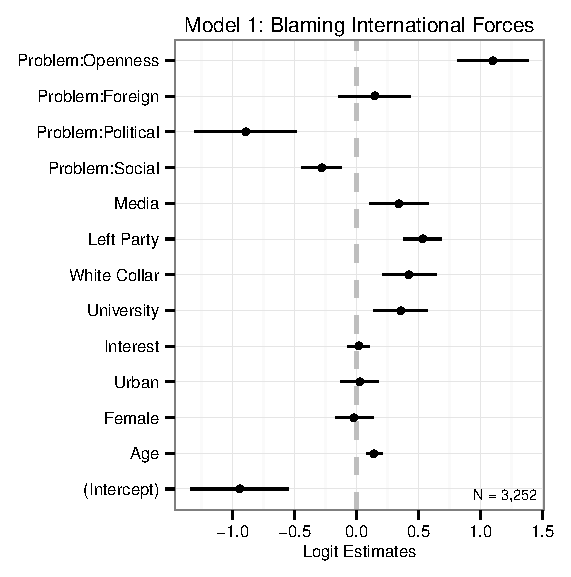
\includegraphics{blame_coefs}
\par\end{centering}

\caption{Direct Effect of Mass Media on Blaming International Forces}
\end{figure}
As logit estimates are not readily interpretable, I simulate the direct
marginal effect of mass media on blame attribution. Figure 4 plots
how a typical respondent's main source of information affects the
probability they will blame international forces.%
\footnote{``Typical'' respondent refers to a female between the ages of 35
and 49, who is a left-party voter, without a bachelor's degree. %
} The effect is small, increasing the probability of blaming international
forces by less than one tenth of a point, but it is statistically
distinguishable from zero at a 95\% confidence level. Similarly, the
indirect effect of mass media on blame, through its effects on perceptions
of openness, is only slightly larger than the direct effect. \pagebreak{}

\begin{center}
\begin{figure}
\begin{centering}
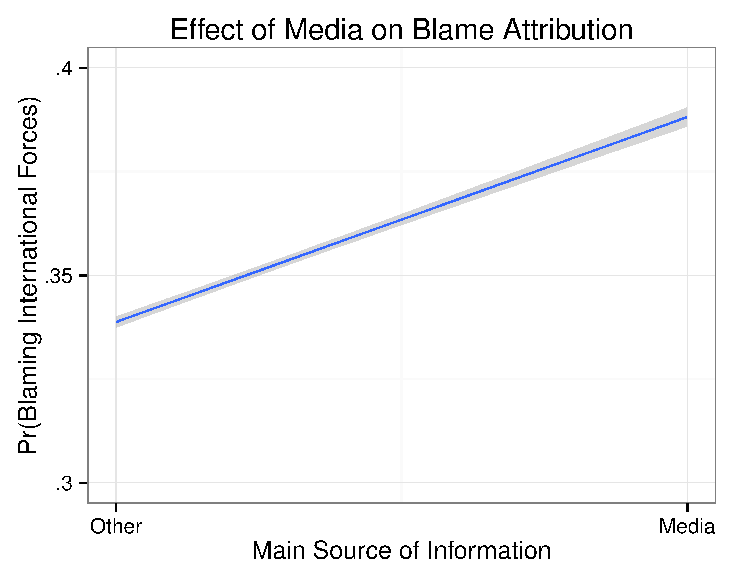
\includegraphics{media_blame_effect}
\par\end{centering}

\caption{Direct Effect of Mass Media on Blame. 95\% confidence intervals in
grey.}
\end{figure}

\par\end{center}

The coefficient plot and simulated probabilities in Figures 5 and
6 reveal statistical evidence for the expectation that blaming international
forces, in turn, has a positive effect on evaluations of the government.%
\footnote{There is reason to suppose that blame attributions could be endogenous
to evaluations of how the government is handling a problem, in the
sense that poor or satisfactory government handling could actually
increase or decrease the government's culpability. First, however,
it should be recalled that survey question I am using to measure blame
attributions refers specifically to the cause of the problem. Thus,
strictly speaking, evaluations of how the government handles the problem
should not affect who or what individuals identify as the cause or
source of the problem. Second, it is much harder to believe that evaluations
of government handling could drive individuals' blame of international
forces or blame of the two alternative targets from which respondents
were able to choose (individuals ``like you and I'' or social institutions)
simply because it is hard to imagine how government handling of the
problem could make any of these other targets more or less culpable.
Thus, I estimate an additional model which has separate binary independent
variables for blaming government, international forces, or ``other''
as the baseline (see Online Appendix). The coefficient for blaming
government is larger than that for blaming international forces but
both remain signed as expected and significant. This alternative specification
mitigates the possibility that blaming international forces merey
reflects (endogenously) respondents who are less likely to blame the
government. Finally, if it can be assumed that endogeneity between
evaluations of handling and blame would be most likely among partisans,
then the control for partisanship and the two separate controls for
support of President Mitterand likely absorb much of this endogeneity.%
}

\begin{center}
\begin{figure}
\begin{centering}
\includegraphics{\string"/Users/Justin/Dropbox/Data General/Article1/govhandling_coefs\string".eps}
\par\end{centering}

\caption{Effects of Blame on Evaluations of the Government}
\end{figure}

\par\end{center}

Figure 6 shows the simulated effect on evaluations of the government's
handling of a problem from shifting their blame for that problem from
the government toward international forces (Hypothesis 2).%
\footnote{These results also hold when the dependent variable refers to satisfaction
with the President. See appendix. %
} The typical respondent would be expected to increase their evaluation
of the government (on a four point scale) about .25 points after a
shift in blame toward international forces.

\begin{center}
\begin{figure}
\begin{centering}
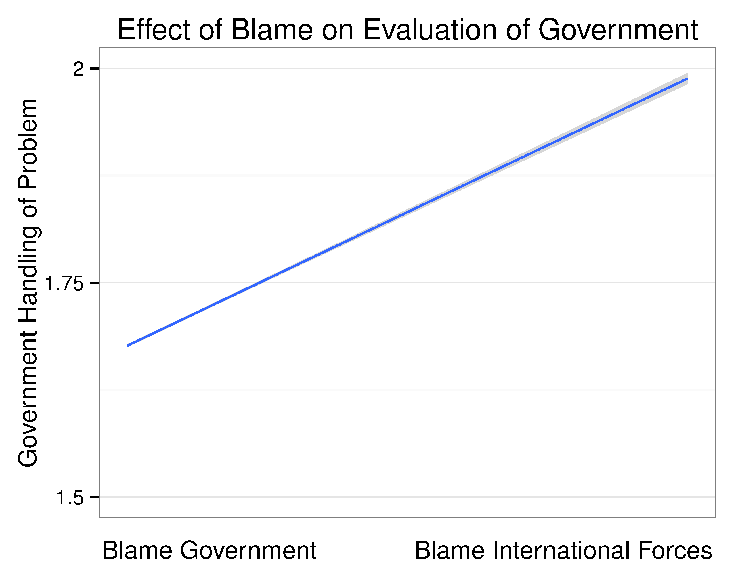
\includegraphics{govhandling_effect}
\par\end{centering}

\caption{Based on 1000 simulations. 95\% confidence intervals in grey.}
\end{figure}

\par\end{center}

Consistent with the evidence in favor of Hypothesis 2, Figures 7 and
8 suggest evidence for the predicted, interactive effects of perceptions
of openness and blame for openness on voter turnout. Whereas perceptions
of openness as a problem and blaming international forces for that
problem both have positive correlations with voter turnout (only the
latter is statistically significant), their interaction has a negative
and statistically significant effect. The logit estimate for the multiplicative
interaction of Problem:Openness\emph{ }and\emph{ }Blame International
is .98 with a standard error of .04\emph{. }Again, the size of the
effect is small, but this is largely because the unconditional probability
that a respondent intends to vote is very high.

\begin{center}
\begin{figure}
\begin{centering}
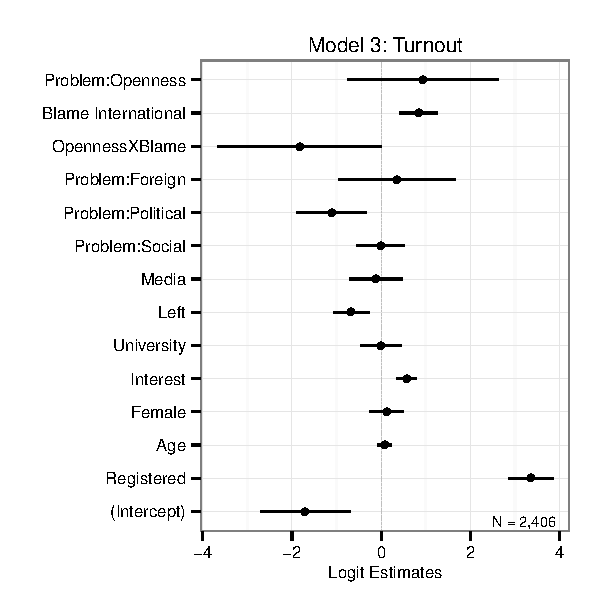
\includegraphics{turnout_coefs}
\par\end{centering}

\caption{The Effect of the Interaction of Openness and Blame on Voter Turnout}
\end{figure}

\par\end{center}

\begin{center}
\begin{figure}
\begin{centering}
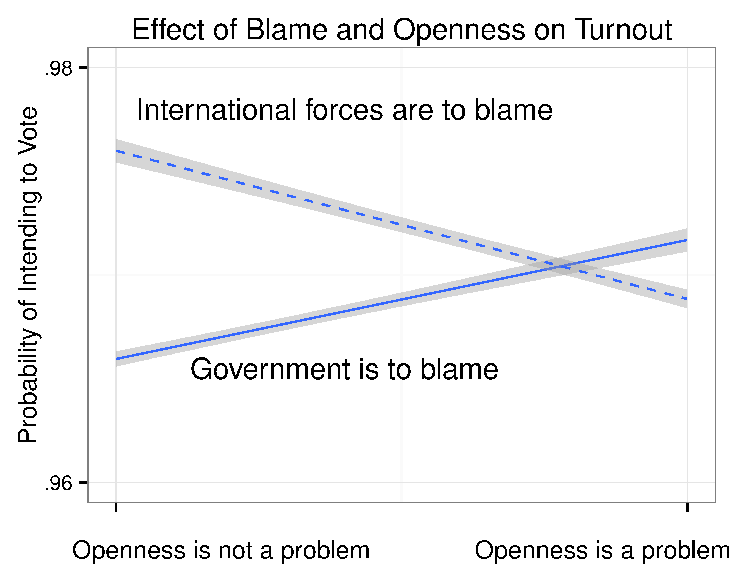
\includegraphics{turnout}
\par\end{centering}

\caption{Based on 1000 simulations. 95\% confidence intervals in grey.}
\end{figure}

\par\end{center}

\pagebreak{}Table 1 displays results from three regression models
which provide initial support for the state-level expectations regarding
the effect of mass media on the globalization-welfare relationship.
In each of the three model specifications, the variable Trade{*}MDI
is negative and statistically significant, suggesting that media density
decreases the effect that trade has on government consumption expenditure.
Before the analysis, all variables were de-meaned and divided by two
standard deviations so that the coefficient for any independent variable
can be interpreted as the expected effect of a two standard deviation
increase in that variable. In other words, the coefficient of -.97
for Trade{*}MDI in Model 1 suggests that, on average, a two standard
deviation increase in media density (109.3 points) in the long-run
decreases the effect that a two standard deviation increase in trade
openness (85.2\% of GDP) has on government spending by .97\% of GDP.
Model 3 estimates that this negative conditioning effect of media
density is as little as .61\% of GDP. Moving from the minimum density
of media (0) to the maximum in the sample (313.3) is associated, on
average, with a decrease of as much as 2.78\%, and as little as 1.8\%,
in the expected effect of an 85\% increase in trade openness on government
spending as a share of GDP. Although the estimated effect appears
relatively slight, it should be kept in mind that the mean level of
government consumption expenditure in the sample is only 15.7\% of
GDP. Thus, for a country that begins with no mass media and becomes
as fully penetrated as the most penetrated (the United States in 1986),
the roughly 1-3\% of GDP by which we would expect the country to reduce
its compensatory public spending in the long-run for an 85\% increase
in trade openness is a substantial portion of what a typical country
spends.

Models 1 and 2 consider variable levels only, while Model 3 is an
error-correction model using first-differences or year-to-year changes
in the dependent variable and lagged levels of the dependent variable
on the right-hand side of the equation, with levels and first-differences
of the key independent variables. Although a level dependent variable
with a lagged level on the right-hand side is formally equivalent
to a differenced dependent variable, the error-correction specification
is useful here because it allows us to separate short-run and long-run
effects.%
\footnote{The error-correction specification is useful here for another reason.
Although government spending and media density are not quite co-integrated,
they are nearly cointegrated as both trend upward over time. In such
situations, error-correction specifications are ideal for insuring
against the possibility of spurious correlations driven by that shared
integration. %
} The differenced independent variables reflect immediate, short-run
effects and the level independent variables reflect the long-run effect
after the short-run effects decay. All three models include fixed
effects for country and year to account for unobserved differences
in countries or unobserved temporal shocks in any particular year.
To control for the clustering of errors within countries and the possibility
of downwardly biased standard errors, I subsequently calculated panel-corrected
standard errors following Beck and Katz \citeyearpar{Anonymous:DMdF8icE}.
Panel-corrected standard errors did not appreciably change the statistical
significance of any estimates reported in this paper.%
\footnote{It is common to display the panel-corrected standard errors rather
than the untransformed errors, but it is not obvious that treating
them as a default has improved our use of cross-sectional, time-series
data. On this point, see\citealt{Wilson:2007kz}, with whom I take
the view that panel-corrected standard errors are only one of many
checks against difficulties common in cross-sectional, time-series
data. Fixed effects, lagged dependent variables, and dynamic specifications
are some of the other techniques stressed by those authors. Here,
I employ all of these techniques, and in some cases all together.%
}

Columns 2 and 3 test the conditioning effect of media density against
the conditioning effects of democracy on the trade-welfare relationship,
which previous research has found to increase the redistributive responsiveness
of domestic welfare spending to international trade (\citealt{Adsera:2002vt}),
suggests that media density has a robust conditioning effect on the
relationship between trade and spending, while the interaction found
by Adser� and Boix no longer appears statistically distinguishable
from zero.

\begin{singlespace}
\noindent \begin{center}
\def\sym#1{\ifmmode^{#1}\else\(^{#1}\)\fi}
\begin{table}[htbp]
\caption {Determinants of Government Consumption Expenditure} \label{tab:title} 
\centering
\footnotesize
\begin{tabular}{l*{3}{c}}
\hline\hline
  &\multicolumn{1}{c}{spending.wb} &\multicolumn{1}{c}{spending.wb} &\multicolumn{1}{c}{diff(spending.wb)} \\
\hline
lag(trade.wb, 1) 		&0.144 		&0.147 		&0.38\sym{*}\\
  		&(0.213) 		&(0.213) 		&(0.222) \\
lag(mdi, 1) 		&-0.157 		&-0.114 		&0.612\sym{*} \\
  		&(0.402) 		&(0.403) 		&(0.318) \\
lag(polity2, 1) 		&0.025 		&-0.03 		& \\
  		&(0.152) 		&(0.157) 		& \\
lag(gdpcap.wb, 1) 		&0.615\sym{***} 		&0.608\sym{***} 		& \\
  		&(0.189) 		&(0.189) 		& \\
lag(dependency.wb, 1) 		&-0.218 		&-0.235 		& \\
  		&(0.231) 		&(0.232) 		& \\
lag(land.wb, 1) 		&13.921 		&20.356 		& \\
  		&(191.648) 		&(191.676) 		& \\
lag(spending.wb, 1) 		&0.717\sym{***} 		&0.716\sym{***} 		&-0.164\sym{***} \\
  		&(0.016) 		&(0.016) 		&(0.01) \\
lag(spending.wb, 2) 		&0.11\sym{***} 		&0.111\sym{***} 		& \\
  		&(0.016) 		&(0.016) 		& \\
lag(trade.wb, 1):lag(mdi, 1) 		&-0.97\sym{***} 		&-0.883\sym{***} 		&-0.611\sym{*} \\
  		&(0.32) 		&(0.325) 		&(0.317) \\
lag(diff(trade.wb)):lag(diff(mdi)) 		& 		& 		&8.139 \\
  		& 		& 		&(15.681) \\
lag(trade.wb, 1):lag(polity2, 1) 		& 		&-0.428 		&-0.434 \\
  		& 		&(0.303) 		&(0.294) \\
lag(diff(trade.wb)):lag(diff(polity2)) 		& 		& 		&-3.557\sym{*} \\
  		& 		& 		&(1.963) \\
lag(diff(trade.wb), 1) 		& 		& 		&-0.946\sym{**} \\
  		& 		& 		&(0.388) \\
lag(diff(mdi), 1) 		& 		& 		&0.562 \\
  		& 		& 		&(1.716) \\
lag(diff(polity2), 1) 		& 		& 		&-0.056 \\
  		& 		& 		&(0.284) \\
lag(diff(gdpcap.wb), 1) 		& 		& 		&0.668 \\
  		& 		& 		&(0.723) \\
lag(diff(dependency.wb), 1) 		& 		& 		&2.4 \\
  		& 		& 		&(1.794) \\
lag(diff(spending.wb), 1) 		& 		& 		&-0.104\sym{***} \\
  		& 		& 		&(0.016) \\
\hline
$R^2$ 		&0.672 		&0.672 		&0.104 \\
$adj.R^2$ 		&0.638 		&0.638 		&0.098 \\
$N$ 		&\multicolumn{1}{c}{3911} 		&\multicolumn{1}{c}{3911} 		&\multicolumn{1}{c}{3914} \\
\hline\hline
\multicolumn{4}{l}{\footnotesize Standard errors in parentheses}\\
\multicolumn{4}{l}{\footnotesize $^{*}$ (p $\le$ 0.1), $^{**}$ (p $\le$ 0.05), $^{***}$ (p $\le$ 0.01)}\\
\end{tabular}
\end{table}

\par\end{center}
\end{singlespace}


\subsection{Rival Explanations}

To check for the possibility that the above models are spuriously
driven by some different but unobserved process distinct from the
effects of mass media, I gather additional data to test my arguments
against a series of rival explanations. Specifically, it is argued
that left parties and union density are aspects of the domestic institutional
environment which lead to more redistributive responses to economic
liberalization (\citealt[674]{Garrett:1995tj}); that electoral systems
defined by proportional representation are more redistributive than
majoritarian systems (\citealt{Iversen:2006wd}); and that the degree
of unitarism or government centralization affects welfare spending
(\citealt[72]{Crepaz:1998vj}). Finally, of particular interest in
the literature relating economic globalization to the politics of
welfare is the argument of Iversen (\citeyear{Iversen:2001vr}) and
Iversen and Cusack (\citeyear{Iversen:2000ch}) that deindustrialization
rather than globalization has driven the expansion of welfare spending
since the 1960s.

In Table 2, I re-estimate the error-correction model (as in Column
3 of Table 1) controlling for each of the rival explanations above.%
\footnote{See Supporting Information for more information on variable descriptions
and sources.%
} The interaction of trade levels and media density levels is robust
to the inclusion of each potentially confounding variable, suggesting
that the conditioning effect of media density on the trade-spending
relationship is not a spurious correlation due to an omitted variable.
Rather, the state-level models overall furnish another level of robust
evidence that mass media shape perceptions and blame attributions
around economic globalization in a way that diffuses the domestic
political pressure required for compensatory, redistributive policy
response.

\begin{singlespace}
\noindent \begin{center}
\def\sym#1{\ifmmode^{#1}\else\(^{#1}\)\fi}
\begin{table}[htbp]
\footnotesize
\centering
\caption{Rival Explanations: Electoral System, Centralization, Left Party Seats, Union Density, and De-Industrialization}
\begin{tabular}{l*{5}{c}}
\hline\hline
  &\multicolumn{1}{c}{(1)} &\multicolumn{1}{c}{(2)} &\multicolumn{1}{c}{(3)} &\multicolumn{1}{c}{(4)} &\multicolumn{1}{c}{(5)} \\
\hline
lag(diff(trade.wb), 1) 		&-0.668 		&-0.429 		&-2.431\sym{**} 		&-1.362 		&-1.345\sym{***} \\
  		&(0.458) 		&(0.467) 		&(1.055) 		&(0.879) 		&(0.481) \\
lag(mdi, 1) 		&0.045 		&-0.014 		&-0.278 		&-0.589\sym{**} 		&-0.047 \\
  		&(0.416) 		&(0.416) 		&(0.262) 		&(0.242) 		&(0.677) \\
lag(diff(mdi), 1) 		&0.814 		&0.743 		&2.258\sym{***} 		&2.839\sym{***} 		&-0.919 \\
  		&(1.743) 		&(1.741) 		&(0.775) 		&(0.821) 		&(2.253) \\
lag(gdpcap.wb, 1) 		&0.472\sym{**} 		&0.509\sym{***} 		&0.556\sym{***} 		&0.427\sym{***} 		&0.833\sym{***} \\
  		&(0.187) 		&(0.187) 		&(0.137) 		&(0.117) 		&(0.285) \\
lag(spending.wb, 1) 		&-0.233\sym{***} 		&-0.234\sym{***} 		&-0.071\sym{***} 		&-0.075\sym{***} 		&-0.247\sym{***} \\
  		&(0.014) 		&(0.014) 		&(0.018) 		&(0.015) 		&(0.013) \\
lag(trade.wb, 1):lag(mdi, 1) 		&-0.662\sym{*} 		&-0.641\sym{**} 		&-0.891\sym{**} 		&-1.184\sym{***} 		&-1.919\sym{***} \\
  		&(0.342) 		&(0.324) 		&(0.354) 		&(0.314) 		&(0.542) \\
lag(diff(trade.wb), 1):lag(diff(mdi), 1) 		&5.072 		&4.268 		&-39.462 		&-41.014 		&41.667\sym{*} \\
  		&(18.142) 		&(18.194) 		&(25.394) 		&(25.531) 		&(25.254) \\
lag(pr, 1) 		&0.476 		& 		& 		& 		& \\
  		&(0.359) 		& 		& 		& 		& \\
lag(trade.wb, 1):lag(pr, 1) 		&0.296 		& 		& 		& 		& \\
  		&(0.334) 		& 		& 		& 		& \\
lag(diff(trade.wb), 1):lag(diff(pr), 1) 		&-11.343\sym{***} 		& 		& 		& 		& \\
  		&(3.858) 		& 		& 		& 		& \\
lag(unitarism, 1) 		& 		&-0.695 		& 		& 		& \\
  		& 		&(0.681) 		& 		& 		& \\
lag(trade.wb, 1):lag(unitarism, 1) 		& 		&0.651 		& 		& 		& \\
  		& 		&(0.536) 		& 		& 		& \\
lag(diff(trade.wb), 1):lag(diff(unitarism), 1) 		& 		&-12.632\sym{*} 		& 		& 		& \\
  		& 		&(6.579) 		& 		& 		& \\
lag(netden, 1) 		& 		& 		&-0.086 		& 		& \\
  		& 		& 		&(0.167) 		& 		& \\
lag(trade.wb, 1):lag(netden, 1) 		& 		& 		&-0.8\sym{**} 		& 		& \\
  		& 		& 		&(0.393) 		& 		& \\
lag(diff(trade.wb), 1):lag(diff(netden), 1) 		& 		& 		&-14.819 		& 		& \\
  		& 		& 		&(21.369) 		& 		& \\
lag(lefts, 1) 		& 		& 		& 		&0.208\sym{*} 		& \\
  		& 		& 		& 		&(0.125) 		& \\
lag(trade.wb, 1):lag(lefts, 1) 		& 		& 		& 		&0.441 		& \\
  		& 		& 		& 		&(0.343) 		& \\
lag(diff(trade.wb), 1):lag(diff(lefts), 1) 		& 		& 		& 		&-2.568 		& \\
  		& 		& 		& 		&(4.755) 		& \\
lag(industry.wb, 1) 		& 		& 		& 		& 		&0.06 \\
  		& 		& 		& 		& 		&(0.253) \\
lag(diff(industry.wb), 1) 		& 		& 		& 		& 		&-0.862\sym{*} \\
  		& 		& 		& 		& 		&(0.517) \\
lag(mdi, 1):lag(industry.wb, 1) 		& 		& 		& 		& 		&0.495 \\
  		& 		& 		& 		& 		&(0.56) \\
lag(diff(mdi), 1):lag(diff(industry.wb), 1) 		& 		& 		& 		& 		&56.869\sym{**} \\
  		& 		& 		& 		& 		&(25.815) \\
\hline
$R^2$ 		&0.125 		&0.123 		&0.194 		&0.147 		&0.144 \\
$adj.R^2$ 		&0.115 		&0.114 		&0.17 		&0.131 		&0.134 \\
$N$ 		&\multicolumn{1}{c}{2224} 		&\multicolumn{1}{c}{2224} 		&\multicolumn{1}{c}{544} 		&\multicolumn{1}{c}{673} 		&\multicolumn{1}{c}{2736} \\
\hline\hline
\multicolumn{6}{l}{\footnotesize Standard errors in parentheses. For space constraints, estimates for land, dependency rates, levels of trade}\\
\multicolumn{6}{l}{\footnotesize and democracy are included but not displayed (all were indistinguishable from zero at 95\% confidence).}\\
\multicolumn{6}{l}{\footnotesize $^{*}$ (p $\le$ 0.1), $^{**}$ (p $\le$ 0.05), $^{***}$ (p $\le$ 0.01)}\\
\end{tabular}
\end{table}

\par\end{center}
\end{singlespace}


\section{{\normalsize{Conclusion}}}

This study has presented individual- and state-level evidence that
mass media functions as a political institution which conditions the
domestic politics of economic globalization. Because politicians use
mass media to avoid blame, mass media decrease the accountability
of national economic policymakers who pursue liberalization. Survey
evidence shows that individuals most reliant on mass media are less
likely to blame incumbent governments for problems wrought by economic
liberalization. Mass media \emph{indirectly} deflects blame away from
incumbent governments by making individuals more aware of economic
openness as a political issue, but it also \emph{directly} decreases
individuals' propensities to blame incumbents (controlling for the
awareness effect), most likely due to framing effects inherent in
mass media. Cross-sectional, time-series data reveal that mass media
is associated with a decrease in the relationship between economic
openness and welfare-state spending, providing further evidence that
mass media diffuses the domestic political pressure against liberalization
that has historically elicited welfare-state compensation for aggreived
domestic groups. The state-level evidence is consistent with the individual-level
evidence that mass media shifts blame attributions away from governments
and toward unaccountable international forces, which in turn allows
national economic policymakers to neglect welfare-state compensation
of harmed domestic groups.

\pagebreak{}

\bibliographystyle{plainnat}
\bibliography{bib}


\pagebreak{}


\subsection{{\normalsize{Supporting Information}}}


\subsection*{{\normalsize{Contents}}}

\noindent Text of Key Survey Questions

\noindent Descriptive Statistics for Survey Data

\noindent Additional Individual-Level Model Results Referenced in
Paper

\noindent State-Level Variable Descriptions

\noindent Descriptive Statistics for State-Level Data


\subsection*{{\normalsize{Text of Key Survey Questions}}}

\textbf{Variable: Media}

\noindent Q-15. (ASK IN EVEN NUMBERED WAVES ONLY: Thinking about what
is going on in our country today, which ONE of the following is the
most important source of information for you? (Interviewer: Ask in
Rotating Order; Circle First Response Only).

1. Family

2. Co-workers and friends

3. Opinion leaders (e.g., religious leaders, teachers, government
officials)

4. The media (TV, radio, newspapers, magazines) 5. None (Volunteered
Only)

6. Other (Volunteered Only)

7. Don\textquoteright{}t Know/No Response (Column 23)

\noindent \textbf{Variable: First and Second Most Important Problem}
(After the respondent selects an issue area, they are given a list
of specific problems from which they can identify the top problem.
See full codebook for the complete list of problems provided.)

\noindent Q-22. What in your opinion is the top problem facing France
today? (Interviewer: Record One Response, Circle One Pre-Coded Reponse
Only; First Mention).

\noindent Q-27. What in your opinion is the second most important
problem facing France today? (Interviewer: Record One Response, Circle
One Pre-Coded Response Only; First Mention).

1. Social Issues (Go To Q.23)

2. Economic Issues (Go To Q.24)

3. Political Issues (Go to Q.25)

4. Foreign Affairs (Go to Q.26)

5. Other (Specify):

6. Don\textquoteright{}t Know/No Response (Column 31)


\subsubsection*{Variable: Blame}

Q-32. Which ONE of the following statements do you think best describes
the cause of the second most important problem you just mentioned?
(Interviewer: Read Statements in Rotating Order; Press Respondent
to Make One Choice Only; Ask if They Have Anything Specific in Mind).
(Note: This question referred to the top problem in Waves 1 and 2
and the second problem from Wave 3 forwards. )

1. ``The cause Iies in the behavior and attitudes of people like
you and me.''

2. ``The cause Iies in our society, that is our institutions and
enterprises.''

3. ``The cause lies in the current policies of the Government.''

4. ``The cause lies in international affairs and is beyond the control
of our country.''

5. Don\textquoteright{}t Know/No Response (Column 49)

Specific Mention: 


\subsubsection*{Variable: Government Handling}

Q-33. How would you rate the performance of the Government in handling
the second most important problem that you just mentioned? Are you...
(Note: This question referred to the top problem in Waves 1 and 2
and the second problem from Wave 3 forwards.)

1. Completely satisfied?

2. Somewhat satisfied?

3. Somewhat dissatisfied?

4. Completely dissatisfied?

5. Don\textquoteright{}t Know/No Response? (Column 50)

\noindent \textbf{Variable: Presidential Satisfaction}

\noindent Q-20. How do you feel about the performance, overall, of
President Mitterand? Are you completely satisfied, somewhat satisfied,
somewhat dissatisfied or completely dissatisfied?

1. Completely satisfied

2. Somewhat satisfied

3. Somewhat dissatisfied

4. Completely dissatisfied

5. Don\textquoteright{}t Know/NoResponse (Column 29)


\subsection*{{\normalsize{Descriptive Statistics for Survey Data}}}

\footnotesize
\begin{longtable}{lrrrrrrrrrr}  \textbf{Variable} & $\mathbf{n}$ & \textbf{Min} & $\mathbf{q_1}$ & $\mathbf{\widetilde{x}}$ & $\mathbf{\bar{x}}$ & $\mathbf{q_3}$ & \textbf{Max} & $\mathbf{s}$ & \textbf{IQR} & \textbf{\#NA} \\    \hline x.age & 29009 & 1 & 2 & 3 & 3.1 & 4 & 5 & 1.3 & 2 &    0 \\    x.interest & 28997 & 1 & 2 & 2 & 2.3 & 3 & 4 & 0.9 & 1 &   12 \\    x.pressat & 26911 & 1 & 2 & 2 & 2.2 & 3 & 4 & 0.8 & 1 & 2098 \\    x.govhandle & 22559 & 1 & 1 & 2 & 2.0 & 2 & 4 & 0.7 & 1 & 6450 \\    x.newspaper & 29009 & 0 & 0 & 0 & 0.1 & 0 & 1 & 0.3 & 0 &    0 \\    \hline \caption{} \label{} \end{longtable}

\begin{longtable}{ll|rrr}  \textbf{Variable} & \textbf{Levels} & $\mathbf{n}$ & $\mathbf{\%}$ & $\mathbf{\sum \%}$ \\    \hline x.registered & no & 1568 & 5.4 & 5.4 \\     & yes & 27441 & 94.6 & 100.0 \\     \hline  & all & 29009 & 100.0 &  \\     \hline \hline x.gender & Male & 13891 & 47.9 & 47.9 \\     & Female & 15118 & 52.1 & 100.0 \\     \hline  & all & 29009 & 100.0 &  \\     \hline \hline x.urban & Not Urban & 16095 & 55.5 & 55.5 \\     & Urban & 12914 & 44.5 & 100.0 \\     \hline  & all & 29009 & 100.0 &  \\     \hline \hline x.college & No university & 12465 & 75.7 & 75.7 \\     & University & 4011 & 24.3 & 100.0 \\     \hline  & all & 16476 & 100.0 &  \\     \hline \hline x.occ & Not white collar & 17059 & 78.6 & 78.6 \\     & White collar & 4637 & 21.4 & 100.0 \\     \hline  & all & 21696 & 100.0 &  \\     \hline \hline x.turnoutint & No & 2036 & 9.1 & 9.1 \\     & Yes & 20241 & 90.9 & 100.0 \\     \hline  & all & 22277 & 100.0 &  \\     \hline \hline x.turnout88 & no & 2729 & 13.0 & 13.0 \\     & yes & 18294 & 87.0 & 100.0 \\     \hline  & all & 21023 & 100.0 &  \\     \hline \hline x.leftcand & Not left & 4931 & 45.5 & 45.5 \\     & Left & 5899 & 54.5 & 100.0 \\     \hline  & all & 10830 & 100.0 &  \\     \hline \hline x.leftparty & Not left & 11558 & 45.2 & 45.2 \\     & Left & 14001 & 54.8 & 100.0 \\     \hline  & all & 25559 & 100.0 &  \\     \hline \hline x.infosource & family & 708 & 4.6 & 4.6 \\     & friends & 791 & 5.1 & 9.7 \\     & opinion leaders & 303 & 2.0 & 11.7 \\     & the media & 13606 & 88.3 & 100.0 \\     \hline  & all & 15408 & 100.0 &  \\     \hline \hline x.media & Other & 1802 & 11.7 & 11.7 \\     & Media & 13606 & 88.3 & 100.0 \\     \hline  & all & 15408 & 100.0 &  \\     \hline \hline x.tv & Other & 7332 & 47.2 & 47.2 \\     & TV & 8194 & 52.8 & 100.0 \\     \hline  & all & 15526 & 100.0 &  \\     \hline \hline x.radio & Other & 13300 & 85.7 & 85.7 \\     & Radio & 2226 & 14.3 & 100.0 \\     \hline  & all & 15526 & 100.0 &  \\     \hline \hline x.magazines & Other & 14784 & 95.2 & 95.2 \\     & Magazines & 742 & 4.8 & 100.0 \\     \hline  & all & 15526 & 100.0 &  \\     \hline \hline x.openprob1 & 0 & 21358 & 96.0 & 96.0 \\     & 1 & 888 & 4.0 & 100.0 \\     \hline  & all & 22246 & 100.0 &  \\     \hline \hline x.openprob2 & 0 & 19880 & 92.4 & 92.4 \\     & 1 & 1627 & 7.6 & 100.0 \\     \hline  & all & 21507 & 100.0 &  \\     \hline \hline x.econprob1 & Other & 25384 & 89.0 & 89.0 \\     & Economic & 3153 & 11.1 & 100.0 \\     \hline  & all & 28537 & 100.0 &  \\     \hline \hline x.socialprob1 & Other & 4499 & 15.8 & 15.8 \\     & Social & 24038 & 84.2 & 100.0 \\     \hline  & all & 28537 & 100.0 &  \\     \hline \hline x.polprob1 & Other & 27885 & 97.7 & 97.7 \\     & Political & 652 & 2.3 & 100.0 \\     \hline  & all & 28537 & 100.0 &  \\     \hline \hline x.foreignprob1 & Foreign & 694 & 2.4 & 2.4 \\     & Other & 27843 & 97.6 & 100.0 \\     \hline  & all & 28537 & 100.0 &  \\     \hline \hline x.econprob2 & Other & 16465 & 66.4 & 66.4 \\     & Economic & 8317 & 33.6 & 100.0 \\     \hline  & all & 24782 & 100.0 &  \\     \hline \hline x.socialprob2 & Other & 10958 & 44.2 & 44.2 \\     & Social & 13824 & 55.8 & 100.0 \\     \hline  & all & 24782 & 100.0 &  \\     \hline \hline x.polprob2 & Other & 23880 & 96.4 & 96.4 \\     & Political & 902 & 3.6 & 100.0 \\     \hline  & all & 24782 & 100.0 &  \\     \hline \hline x.foreignprob2 & Foreign & 1739 & 7.0 & 7.0 \\     & Other & 23043 & 93.0 & 100.0 \\     \hline  & all & 24782 & 100.0 &  \\     \hline \hline x.allcauses & personal choices & 3326 & 14.2 & 14.2 \\     & society & 5301 & 22.7 & 36.9 \\     & government & 6694 & 28.6 & 65.5 \\     & outside forces & 7497 & 32.1 & 97.6 \\     & other & 558 & 2.4 & 100.0 \\     \hline  & all & 23376 & 100.0 &  \\     \hline \hline x.cause.gov & not government & 16682 & 71.4 & 71.4 \\     & government & 6694 & 28.6 & 100.0 \\     \hline  & all & 23376 & 100.0 &  \\     \hline \hline x.cause.intl & not international & 15879 & 67.9 & 67.9 \\     & international & 7497 & 32.1 & 100.0 \\     \hline  & all & 23376 & 100.0 &  \\     \hline \hline x.causes & government & 6694 & 47.2 & 47.2 \\     & outside forces & 7497 & 52.8 & 100.0 \\     \hline  & all & 14191 & 100.0 &  \\     \hline \hline \hline \caption{} \label{} \end{longtable}


\subsection*{{\normalsize{\pagebreak{}}}}


\subsection*{{\normalsize{Additional Individual-Level Model Results}}}


\subsubsection*{Results Table for Model 1: Effects of Mass Media on Blame Attributions}

\begin{center}
\begin{table}[!ht]
\caption{}
\label{} 
\begin{tabular}{ l D{.}{.}{2}D{.}{.}{2} }

\hline 
  & \multicolumn{ 2 }{ c }{ Model 1 } \\ \hline

(Intercept)               & -0.94 ^*                  & (0.20)                   \\ 
Age                       & 0.14 ^*                   & (0.03)                   \\ 
genderFemale              & -0.02                     & (0.08)                   \\ 
urbanUrban                & 0.03                      & (0.08)                   \\ 
Interest                  & 0.02                      & (0.04)                   \\ 
collegeUniversity         & 0.36 ^*                   & (0.11)                   \\ 
occWhite Collar           & 0.43 ^*                   & (0.11)                   \\ 
leftpartyLeft Party       & 0.53 ^*                   & (0.08)                   \\ 
mediaMedia                & 0.35 ^*                   & (0.12)                   \\ 
genprob2Problem:Social    & -0.28 ^*                  & (0.08)                   \\ 
genprob2Problem:Political & -0.89 ^*                  & (0.20)                   \\ 
genprob2Problem:Foreign   & 0.15                      & (0.15)                   \\ 
openprob2Problem:Openness & 1.10 ^*                   & (0.14)                   
\\

$N$       & \multicolumn{2}{c}{3252    }\\ 
AIC       & \multicolumn{2}{c}{4206.90 }\\ 
BIC       & \multicolumn{2}{c}{4523.42 }\\ 
$\log L$ & \multicolumn{2}{c}{-2051.45}
\\ \hline

\multicolumn{3}{l}{\footnotesize{Standard errors in parentheses}}\\
\multicolumn{3}{l}{\footnotesize{$^*$ indicates significance at $p< 0.05 $}}

\end{tabular}


\end{table}


\par\end{center}


\subsubsection*{Alternative DV for Model 1: Blame Government vs. Any Other}

\begin{center}
\includegraphics{blame_coefs\lyxdot 1\lyxdot B}
\par\end{center}

\begin{center}
\begin{table}[!ht]
\caption{}
\label{} 
\begin{tabular}{ l D{.}{.}{2}D{.}{.}{2} }

\hline 
  & \multicolumn{ 2 }{ c }{ Model 1 } \\ \hline

(Intercept)               & 0.33                      & (0.17)                   \\ 
Age                       & -0.07 ^*                  & (0.03)                   \\ 
genderFemale              & -0.10                     & (0.07)                   \\ 
urbanUrban                & -0.12                     & (0.07)                   \\ 
Interest                  & -0.02                     & (0.04)                   \\ 
collegeUniversity         & -0.42 ^*                  & (0.09)                   \\ 
occWhite Collar           & -0.38 ^*                  & (0.10)                   \\ 
leftpartyLeft Party       & -0.66 ^*                  & (0.07)                   \\ 
mediaMedia                & -0.30 ^*                  & (0.10)                   \\ 
genprob2Problem:Social    & -0.18 ^*                  & (0.07)                   \\ 
genprob2Problem:Political & 0.44 ^*                   & (0.17)                   \\ 
genprob2Problem:Foreign   & -0.12                     & (0.14)                   \\ 
openprob2Problem:Openness & -0.98 ^*                  & (0.14)                   
\\

$N$       & \multicolumn{2}{c}{5148    }\\ 
AIC       & \multicolumn{2}{c}{5771.77 }\\ 
BIC       & \multicolumn{2}{c}{6112.18 }\\ 
$\log L$ & \multicolumn{2}{c}{-2833.88}
\\ \hline

\multicolumn{3}{l}{\footnotesize{Standard errors in parentheses}}\\
\multicolumn{3}{l}{\footnotesize{$^*$ indicates significance at $p< 0.05 $}}

\end{tabular}


\end{table}


\par\end{center}


\subsubsection*{Alternative DV for Model 1: Blame International vs. Any Other}

\begin{center}
\includegraphics{blame_coefs\lyxdot 1\lyxdot C}
\par\end{center}

\begin{center}
\begin{table}[!ht]
\caption{}
\label{} 
\begin{tabular}{ l D{.}{.}{2}D{.}{.}{2} }

\hline 
  & \multicolumn{ 2 }{ c }{ Model 1 } \\ \hline

(Intercept)               & -1.00 ^*                  & (0.16)                   \\ 
Age                       & 0.12 ^*                   & (0.03)                   \\ 
genderFemale              & -0.10                     & (0.06)                   \\ 
urbanUrban                & -0.10                     & (0.06)                   \\ 
Interest                  & 0.01                      & (0.04)                   \\ 
collegeUniversity         & 0.07                      & (0.08)                   \\ 
occWhite Collar           & 0.20 ^*                   & (0.08)                   \\ 
leftpartyLeft Party       & 0.11                      & (0.06)                   \\ 
mediaMedia                & 0.24 ^*                   & (0.10)                   \\ 
genprob2Problem:Social    & -0.67 ^*                  & (0.07)                   \\ 
genprob2Problem:Political & -0.86 ^*                  & (0.17)                   \\ 
genprob2Problem:Foreign   & 0.09                      & (0.11)                   \\ 
openprob2Problem:Openness & 0.61 ^*                   & (0.10)                   
\\

$N$       & \multicolumn{2}{c}{5148    }\\ 
AIC       & \multicolumn{2}{c}{6466.48 }\\ 
BIC       & \multicolumn{2}{c}{6806.89 }\\ 
$\log L$ & \multicolumn{2}{c}{-3181.24}
\\ \hline

\multicolumn{3}{l}{\footnotesize{Standard errors in parentheses}}\\
\multicolumn{3}{l}{\footnotesize{$^*$ indicates significance at $p< 0.05 $}}

\end{tabular}


\end{table}


\par\end{center}


\subsubsection*{Results Table for Model 1.2: Effects of Mass Media on Perceptions
of Openness as a Problem}

\begin{center}
\begin{table}[!ht]
\caption{}
\label{} 
\begin{tabular}{ l D{.}{.}{2}D{.}{.}{2} }

\hline 
  & \multicolumn{ 2 }{ c }{ Model 1 } \\ \hline

(Intercept)                 & -4.99 ^*                    & (0.31)                     \\ 
foreignprob2Problem:Foreign & 2.79 ^*                     & (0.20)                     \\ 
econprob2Problem:Economic   & 2.92 ^*                     & (0.16)                     \\ 
Age                         & -0.05                       & (0.04)                     \\ 
genderFemale                & -0.30 ^*                    & (0.10)                     \\ 
urbanUrban                  & 0.08                        & (0.10)                     \\ 
Interest                    & 0.17 ^*                     & (0.06)                     \\ 
collegeUniversity           & -0.08                       & (0.13)                     \\ 
occWhite Collar             & 0.41 ^*                     & (0.13)                     \\ 
mitterandMitterand          & 0.22                        & (0.12)                     \\ 
leftpartyLeft Party         & 0.24 ^*                     & (0.12)                     \\ 
mediaMedia                  & 0.44 ^*                     & (0.18)                     
\\

$N$       & \multicolumn{2}{c}{4770    }\\ 
AIC       & \multicolumn{2}{c}{2771.39 }\\ 
BIC       & \multicolumn{2}{c}{3081.96 }\\ 
$\log L$ & \multicolumn{2}{c}{-1337.70}
\\ \hline

\multicolumn{3}{l}{\footnotesize{Standard errors in parentheses}}\\
\multicolumn{3}{l}{\footnotesize{$^*$ indicates significance at $p< 0.05 $}}

\end{tabular}


\end{table}


\par\end{center}


\subsubsection*{Alternative Blame IV for Model 2}

\begin{center}
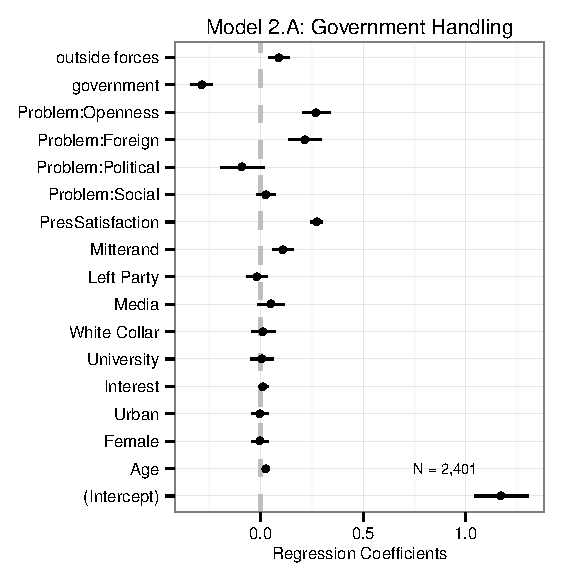
\includegraphics{govhandling_altcause_coefs}
\par\end{center}

\begin{center}
\begin{table}[!ht]
\caption{}
\label{} 
\begin{tabular}{ l D{.}{.}{2}D{.}{.}{2} }

\hline 
  & \multicolumn{ 2 }{ c }{ Model 1 } \\ \hline

(Intercept)               & 1.17 ^*                   & (0.07)                   \\ 
Age                       & 0.03 ^*                   & (0.01)                   \\ 
genderFemale              & -0.00                     & (0.02)                   \\ 
urbanUrban                & -0.00                     & (0.02)                   \\ 
Interest                  & 0.01                      & (0.01)                   \\ 
collegeUniversity         & 0.01                      & (0.03)                   \\ 
occWhite Collar           & 0.01                      & (0.03)                   \\ 
mediaMedia                & 0.05                      & (0.03)                   \\ 
leftpartyLeft Party       & -0.02                     & (0.03)                   \\ 
mitterandMitterand        & 0.11 ^*                   & (0.03)                   \\ 
PresSatisfaction          & 0.27 ^*                   & (0.02)                   \\ 
genprob2Problem:Social    & 0.03                      & (0.02)                   \\ 
genprob2Problem:Political & -0.09                     & (0.05)                   \\ 
genprob2Problem:Foreign   & 0.22 ^*                   & (0.04)                   \\ 
openprob2Problem:Openness & 0.27 ^*                   & (0.03)                   \\ 
causegovernment           & -0.29 ^*                  & (0.03)                   \\ 
causeoutside forces       & 0.09 ^*                   & (0.03)                   
\\

$N$        & \multicolumn{2}{c}{3680}\\ 
$R^2$      & \multicolumn{2}{c}{0.25}\\ 
adj. $R^2$ & \multicolumn{2}{c}{0.25}\\ 
Resid. sd  & \multicolumn{2}{c}{0.62}
\\ \hline

\multicolumn{3}{l}{\footnotesize{Standard errors in parentheses}}\\
\multicolumn{3}{l}{\footnotesize{$^*$ indicates significance at $p< 0.05 $}}

\end{tabular}


\end{table}


\par\end{center}


\subsubsection*{Alternative DV For Model 2: Presidential Satisfaction}

\begin{center}
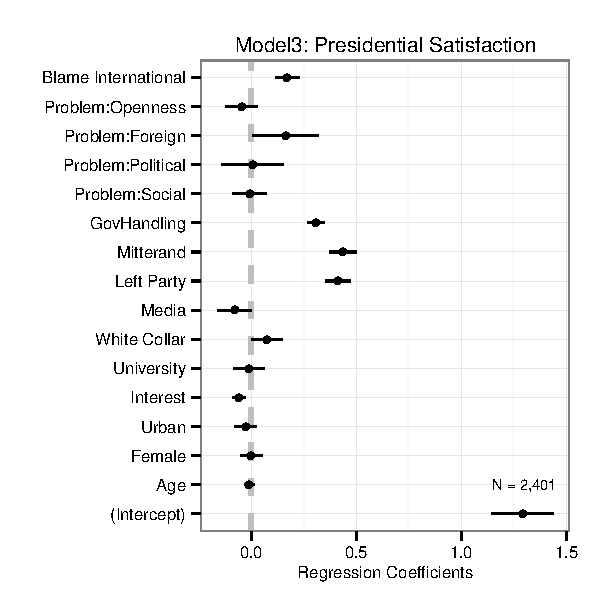
\includegraphics{pressat_coefs}
\par\end{center}

\begin{center}
\begin{table}[!ht]
\caption{}
\label{} 
\begin{tabular}{ l D{.}{.}{2}D{.}{.}{2} }

\hline 
  & \multicolumn{ 2 }{ c }{ Model 1 } \\ \hline

(Intercept)               & 1.29 ^*                   & (0.07)                   \\ 
Age                       & -0.01                     & (0.01)                   \\ 
genderFemale              & -0.00                     & (0.03)                   \\ 
urbanUrban                & -0.03                     & (0.03)                   \\ 
Interest                  & -0.06 ^*                  & (0.02)                   \\ 
collegeUniversity         & -0.01                     & (0.04)                   \\ 
occWhite Collar           & 0.07 ^*                   & (0.04)                   \\ 
mediaMedia                & -0.08                     & (0.04)                   \\ 
leftpartyLeft Party       & 0.41 ^*                   & (0.03)                   \\ 
mitterandMitterand        & 0.44 ^*                   & (0.03)                   \\ 
GovHandling               & 0.31 ^*                   & (0.02)                   \\ 
genprob1Problem:Social    & -0.01                     & (0.04)                   \\ 
genprob1Problem:Political & 0.01                      & (0.07)                   \\ 
genprob1Problem:Foreign   & 0.16 ^*                   & (0.08)                   \\ 
openprob2Problem:Openness & -0.05                     & (0.04)                   \\ 
causesBlame International & 0.17 ^*                   & (0.03)                   
\\

$N$        & \multicolumn{2}{c}{2401}\\ 
$R^2$      & \multicolumn{2}{c}{0.41}\\ 
adj. $R^2$ & \multicolumn{2}{c}{0.41}\\ 
Resid. sd  & \multicolumn{2}{c}{0.62}
\\ \hline

\multicolumn{3}{l}{\footnotesize{Standard errors in parentheses}}\\
\multicolumn{3}{l}{\footnotesize{$^*$ indicates significance at $p< 0.05 $}}

\end{tabular}


\end{table}


\par\end{center}

\pagebreak{}


\subsection*{{\normalsize{State-Level Variable Descriptions}}}

\begin{flushleft}

% latex table generated in R 2.15.2 by xtable 1.7-0 package
% Thu Apr 11 13:27:12 2013
\begin{landscape}
\begin{table}[ht]
\begin{center}
\begin{tabular}{rll}
  \hline
 Variable Name & Description \\ 
  \hline
spending & General government final consumption expenditure as a share of GDP. World Bank.\\ 
trade & Imports + exports as a share of GDP. World Bank.\\ 
dependency & Number of people under 15 and over 64 as a share of working-age population. World Bank. \\ 
land & Land area in square kilometers. World Bank. \\ 
mdi & (Daily newspapers + radio sets + televisions) per 100 people. Arthur Banks and World Bank. See Warren 2012).\\ 
gdpcap & Gross domestic product divided by midyear population (current USD). World Bank. \\ 
polity2 & Democracy - autocracy scores from the Polity IV database. Marshall et al. 2010 \\ 
industry & Value added by industries belonging to manufacturing as share of GDP (ISIC divisions 15-37). World Bank.\\ 
pr & 0 = majoritarian or preferential-vote, 1 = mixed-member majority or bloc vote, 2= list-PR. Gerring and Thacker 2005. \\ 
unitarism & Average of nonfederalism and nonbicameralism. Gerring and Thacker 2005. \\ 
netden & Total union membership weighted by total dependent labor force. Golden et al. 2009. \\ 
lefts & Percentage of seats held by left parties in the legislature. Swank 2006. \\ 
   \hline
\end{tabular}
\end{center}
\end{table}
\end{landscape}

\par\end{flushleft}

\begin{flushleft}
\pagebreak{}
\par\end{flushleft}


\subsection*{{\normalsize{Descriptive Statistics for State-Level Data}}}

\begin{center}
% latex table generated in R 2.15.2 by xtable 1.7-0 package
% Thu Apr 11 12:54:37 2013
\begin{longtable}{lrrrrrrrrrr}
\caption{Descriptive Statistics for State Level Economic Variables} \\
	\textbf{Variable} & $\mathbf{n}$ & \textbf{Min} & $\mathbf{q_1}$ & $\mathbf{\widetilde{x}}$ & $\mathbf{\bar{x}}$ & $\mathbf{q_3}$ &
		\textbf{Max} & $\mathbf{s}$ & \textbf{IQR} & \textbf{\#NA} \\ 
			\hline
scode & 12379 &    2.0 &   155.0 &    350.0 &    375.5 &    572.0 &      950.0 &     247.1 &    417.0 &     0 \\ 
  year & 12379 & 1815.0 &  1893.0 &   1958.0 &   1937.2 &   1983.0 &     2003.0 &      54.6 &     90.0 &     0 \\ 
  polity2 & 12289 &  -10.0 &    -7.0 &     -3.0 &     -0.9 &      6.0 &       10.0 &       7.0 &     13.0 &    90 \\ 
  spending.wb &  4908 &    3.0 &    10.7 &     14.4 &     15.7 &     19.1 &       76.2 &       6.9 &      8.4 &  7471 \\ 
  trade.wb &  5088 &    0.4 &    38.0 &     56.3 &     65.3 &     82.6 &      412.2 &      42.4 &     44.6 &  7291 \\ 
  mdi &  5696 &    0.0 &     8.2 &     23.9 &     46.1 &     66.5 &      313.3 &      53.4 &     58.3 &  6683 \\ 
  gdpcap.wb &  5222 &   37.5 &   306.2 &    849.2 &   3636.2 &   2833.4 &    49263.5 &    6880.6 &   2527.2 &  7157 \\ 
  dependency.wb &  5806 &   30.0 &    58.9 &     81.3 &     76.6 &     91.8 &      112.8 &      18.5 &     33.0 &  6573 \\ 
  land.wb &  5675 &  670.0 & 68890.0 & 248360.0 & 831892.2 & 743530.0 & 16389950.0 & 1843918.4 & 674640.0 &  6704 \\ 
  pr &  2974 &    0.0 &     0.0 &      1.0 &      0.9 &      2.0 &        2.0 &       0.9 &      2.0 &  9405 \\ 
  unitarism &  2973 &    0.0 &     1.0 &      2.0 &      1.5 &      2.0 &        2.0 &       0.7 &      1.0 &  9406 \\ 
  industry.wb &  3718 &    0.2 &     9.0 &     14.5 &     15.1 &     19.9 &       45.3 &       7.7 &     10.9 &  8661 \\ 
  netden &   779 &    0.1 &     0.3 &      0.4 &      0.4 &      0.5 &        0.8 &       0.2 &      0.2 & 11600 \\ 
  lefts &  1010 &    0.0 &    30.0 &     41.0 &     37.0 &     48.9 &       69.6 &      16.2 &     18.9 & 11369 \\ 
  \hline
\label{}
\end{longtable}
\end{landscape}
\par\end{center}
\end{document}
